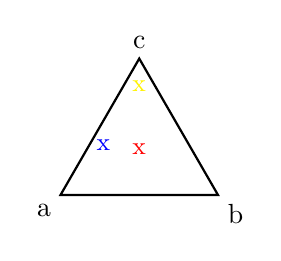
\begin{tikzpicture}
		\coordinate (A) at (0:0);
		\coordinate (B) at (0:2);
		\coordinate (C) at (60:2);
		
		\node[below left] at (A) {a};
		\node[below right] at (B) {b};
		\node[above] at (C) {c};
		
		\draw [thick] (A) -- (B) -- (C) -- cycle;
		
  		\node at (barycentric cs:A=0.33,B=0.33,C=0.33) {\small \textcolor{red}{x}} ;
  		\node at (barycentric cs:A=0.6,B=0.1,C=0.4) {\small \textcolor{blue}{x}} ;
  		\node at (barycentric cs:A=0.1,B=0.1,C=0.8) {\small \textcolor{yellow}{x}} ;
		\end{tikzpicture}
		\quad
		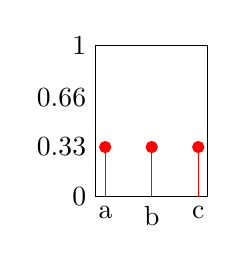
\begin{tikzpicture}
		\begin{axis}[
		width = 3cm,
		height = 3.5cm,
		symbolic x coords={a,b,c},
		xtick=data,
		ytick={0, 0.33, 0.66, 1},
		ymax=1,
		ymin=0,
		ytick style={draw=none},
		xtick style={draw=none}		
		]
		\addplot+[ycomb, color=red, mark options={red}] coordinates {(a,0.33) (b,0.33) (c,0.33)};
		\end{axis}
		\end{tikzpicture}
		\quad
		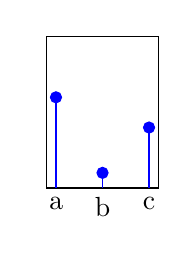
\begin{tikzpicture}
		\begin{axis}[
		width = 3cm,
		height = 3.5cm,
		symbolic x coords={a,b,c},
		xtick=data,
		yticklabels={,,},
		ymax=1,
		ymin=0,
		ytick style={draw=none},
		xtick style={draw=none}		
		]
		\addplot+[ycomb, color=blue, mark options={blue}] coordinates {(a,0.6) (b,0.1) (c,0.4)};
		\end{axis}
		\end{tikzpicture}
		\quad
		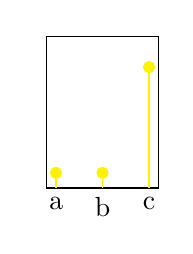
\begin{tikzpicture}
		\begin{axis}[
		width = 3cm,
		height = 3.5cm,
		symbolic x coords={a,b,c},
		xtick=data,
		ymax=1,
		ymin=0,
		ytick style={draw=none},
		xtick style={draw=none},
		yticklabels={,,}		
		]
		\addplot+[ycomb, color=yellow, mark options={yellow}] coordinates {(a,0.1) (b,0.1) (c,0.8)};
		\end{axis}
		\end{tikzpicture}